\section{Software de codificación y decodificación}

\subsection{Pregunta 6 (Codificación heurística)}

\begin{figure}[H]
    \centering
    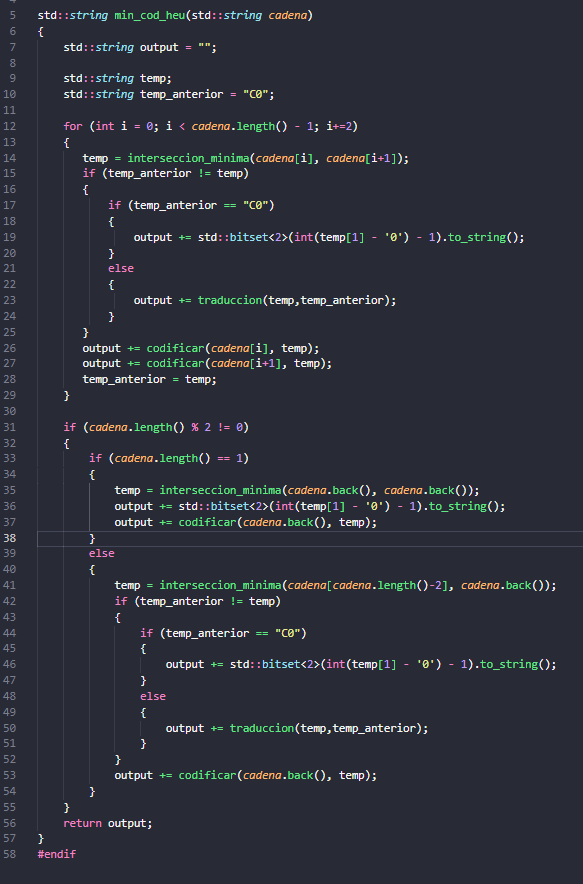
\includegraphics[scale = 0.4]{imagenes/voraz.png}
    \caption{Código en C++ - Algoritmo heurístico}
\end{figure}


\subsection{Pregunta 7 (Codificación óptima)}

\begin{figure}[H]
    \centering
    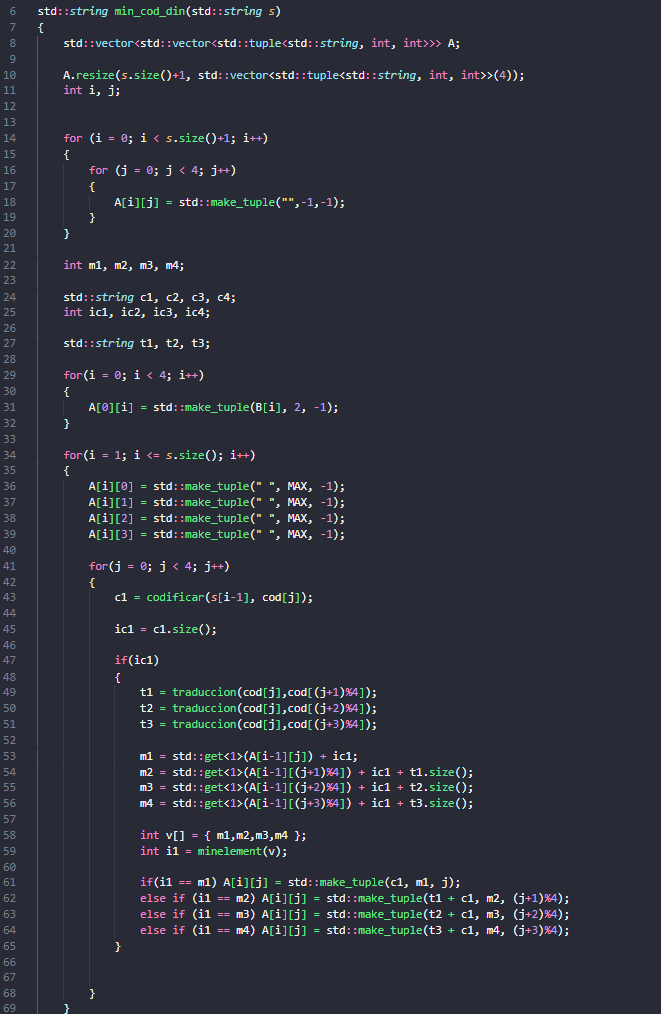
\includegraphics[scale = 0.4]{imagenes/optima.png}
    \caption{Código en C++ - Algoritmo óptimo}
\end{figure}


\subsection{Pregunta 8 (Decodificación)}

\begin{figure}[H]
    \centering
    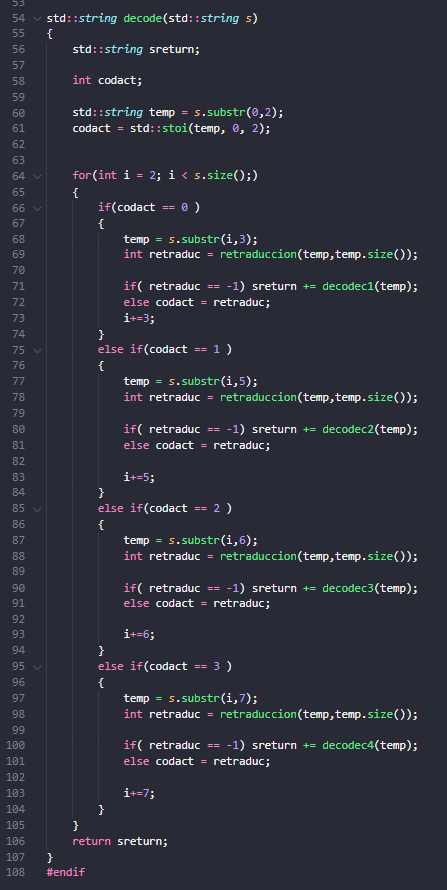
\includegraphics[scale = 0.4]{imagenes/decode.png}
    \caption{Código en C++ - Decodificador}
\end{figure}


\subsection{Pregunta 9 (Software de codificación y decodificación)}

\begin{figure}[H]
    \centering
    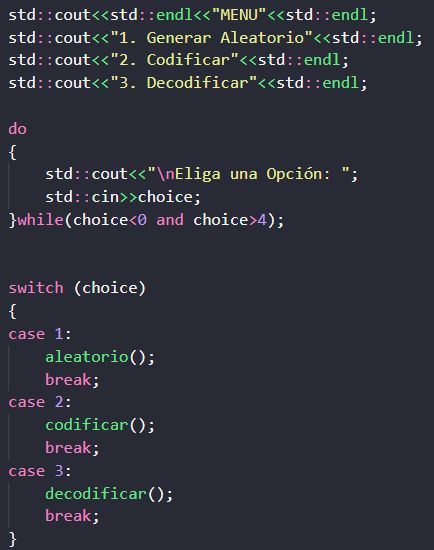
\includegraphics[scale = 0.4]{imagenes/software.png}
    \caption{Menú del software}
\end{figure}

Con el objetivo de que el software sea de utilidad y fácil manejo, se creó un menú del cual
de un archivo recibido realiza:

\begin{itemize}
    \item \textbf{aleatorio()}
    Solicita en consola el tamaño $n$ de la cadena que se creará de manera aleaoria. La longitud máxima puede ser de 1M.
    \item \textbf{codificar()}
    Si se elige esta opción, se recibe un archivo de texto al que se desee codificar, ya sea con un método heurístico u 
    óptimo mínimo. El resultado es guardado como un archivo binario comprimido.
    \item \textbf{decodificar()}
    Se recibe un archivo binario el cual es decodificado y guarda la respuesta en un archivo de texto.
\end{itemize}


\subsection{Pregunta 10 (Análisis experimental)}

Para el analisis experimental, se comparó ambos algoritmos del proyecto con diferentes tamaños de 
tests cases.

\begin{table}[H]
    \begin{tabular}{lll}
    \textbf{Size del encoding} & \textbf{Heurística(ms)} & \textbf{Dinámica(ms)} \\
    10                         & 0.015                   & 0.056                 \\
    100                        & 0.041                   & 0.378                 \\
    1000                       & 0.354                   & 3.737                 \\
    10000                      & 3.252                   & 47.679                \\
    100000                     & 37.132                  & 19123.2               \\
    1000000                    & 299.102                 & 194970               
\end{tabular}
\end{table}
